\documentclass[../../../../main.tex]{subfiles}
\begin{document}

\begin{flushright}
\footnotesize\textit{【自動文字起こし・要確認】}
\end{flushright}

[解] 3回で引くカードは以下のようである。
\begin{center}
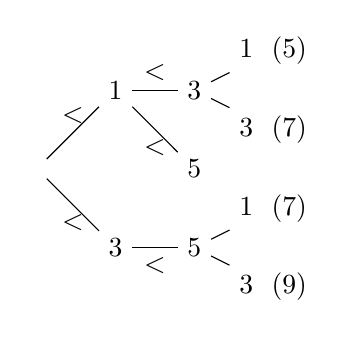
\begin{tikzpicture}
  \node (start) at (0,0) {};
  \node (1) at (1,1) {$1$};
  \node (3) at (1,-1) {$3$};
  \node (13) at (2,1) {$3$};
  \node (15) at (2,0) {$5$};
  \node (35) at (2,-1) {$5$};
  \node (131) at (3,1.5) {$1$ \ (5)};
  \node (133) at (3,0.5) {$3$ \ (7)};
  \node (351) at (3,-0.5) {$1$ \ (7)};
  \node (353) at (3,-1.5) {$3$ \ (9)};
  \draw (start) -- (1) node[midway, above] {$<$};
  \draw (start) -- (3) node[midway, below] {$<$};
  \draw (1) -- (13) node[midway, above] {$<$};
  \draw (1) -- (15) node[midway, below] {$<$};
  \draw (3) -- (35) node[midway, below] {$<$};
  \draw (13) -- (131);
  \draw (13) -- (133);
  \draw (35) -- (351);
  \draw (35) -- (353);
\end{tikzpicture}
\end{center}
(1) A, Bがk点得る確率は以下の通り
\begin{center}
\begin{tabular}{|c|c|c|}
\hline
 & A & B \\ \hline
3 & $p^3$ & $p^3$ \\ \hline
4 & $2p(1-p)$ & 0 \\ \hline
5 & $p^2(1-p)$ & $3p^2(1-p)$ \\ \hline
6 & $(1-p)^2$ & $(1-p)^2$ \\ \hline
0 & 0 & $2p(1-p)^2$ \\ \hline
計 & 1 & 1 \\ \hline
\end{tabular}
\end{center}
したがって、
$$
E_A = 3p^3 + 4 \cdot 2p(1-p) + 5 \cdot p^2(1-p) + 6 \cdot (1-p)^2
$$
$$
= -2p^3 + 3p^2 - 4p + 6
$$
$$
E_B = 3p^3 + 5 \cdot 3p^2(1-p) + 6 \cdot (1-p)^2
$$
$$
= -12p^3 + 21p^2 - 12p + 6
$$
である。又、
$$
E_A > E_B \Leftrightarrow 3p^2 - 4p > -10p^3 + 21p^2 - 12p \Leftrightarrow p(5p-4) < 0 \quad (\because 0 < p < 1)
$$
から、$0 < p < \frac{4}{5}$である。

(2) (1)の表から、Bが何点か（これは排反）で場合分けして、
$$
P_A = \underbrace{2p(1-p)^2}_{\text{Bが0点}} + \underbrace{p^3(1-p^3)}_{\text{Bが3点}} + \underbrace{(1-p)^2 \cdot 3p^2(1-p)}_{\text{Bが5点}}
$$
$$
= p(1-p) \left[ 2(1-p) + p^2(1+p+p^2) + 3p(1-p)^2 \right]
$$
$$
= p(1-p) (p^4 + 4p^3 - 5p^2 + p + 2)
$$
又、全ての事象は、"Aが勝つ" "Bが勝つ" "引き分け" の3つの排反事象で全てだから、
$$
P_B = 1 - P_A - \{ p^3 \cdot p^3 + p^2(1-p) \cdot 3p^2(1-p) + (1-p)^2 \cdot (1-p)^2 \}
$$
$$
= 1 - P_A - \{ p^6 + 3p^4(1-p)^2 + (1-p)^4 \}
$$
である。よって、
$$
P_A > P_B \Leftrightarrow 2P_A > 1 - p^6 - 3p^4(1-p)^2 - (1-p)^4
$$
$$
\Leftrightarrow 2p(1-p)(p^4 + 4p^3 - 5p^2 + p + 2) > 2p(1-p)(2 - p + p^2 - p^3 + 2p^4)
$$
$$
\Leftrightarrow p^4 + 4p^3 - 5p^2 + p + 2 > 2p^4 - p^3 + p^2 - p + 2 \quad (\because 0 < p < 1)
$$
$$
\Leftrightarrow 0 > p(p^3 - 5p^2 + 6p - 2)
$$
$$
\Leftrightarrow 0 > p(p-1)(p^2 - 4p + 2)
$$
\textcircled{1}から言えない。($2-\sqrt{2} < p$)

\end{document}
